\let\oldthesubsection=\thesubsection
\renewcommand{\thesubsection}{\Roman{subsection}}

%A dolgozat olyan nyelvtechnológiai előfeldolgozó algoritmusokat mutat be, melyek hatékonyan képesek szövegek elemzésére agglutináló nyelvek esetén. 
%Vizsgálataimat magyar nyelvre végeztem, de a módszerek kidolgozása során törekedtem a nyelvfüggetlenségre. 
%Így, a bemutatott eljárások más, hasonló struktúrájú nyelvek esetén is sikerrel alkalmazhatóak.
%%Munkám során kiemelt szerep jutott a morfológiai egyértelműsítés feladatának, mivel ennek kimenetére számtalan információkinyerő rendszer épít.
%
%Az első téziscsoportban a általános magyar nyelvű morfológiai egyértelműsítés területén elért eredményeimről számolok be. 
%Ezt követően bemutatom a létrehozott annotáló eszköz egy gyakorlati alkalmazását. 
%Végül, ismertetem azon új előfeldolgozó eljárásokat, melyek zajos (klinikai) szövegeket is hatékonyan képesek elemezni.
%

\subsection{Effective morphological tagging methods for morphologically rich languages} %TODO: igeidők
\label{thes:morf}

Full morphological tagging is a complex task composed of two parts. 
Beside identifying morphosyntactic tags, lemmata of words must be computed as well.
While the first task is a well-known problem of \acrlong{nlp}, the latter one is often neglected.
We start summing our results with the new lemmatization method, following this the full tagging systems are presented. 


\begin{core}
\begin{thesis}\label{thes:morf-lemma}
We developed a new lemmatization method for agglutinative languages.
The presented algorithm is based on the output of a morphological analyzer, however, it can handle both known and unknown words effectively by incorporating diverse models. 
Results presented show that it has superior performance on Hungarian texts.
\end{thesis} 

\begin{pub}
\cite{Orosz2011,Orosz2012,Orosz2012a,Orosz2013a}
\end{pub}
\end{core}

The proposed algorithm performs lemmatization in two steps. 
First, it uses a morphological analyzer to generate lemma candidates, then disambiguation is performed using different stochastic models.
The latter part is carried out calculating the score ($S$) of each lemma ($l$) for a given word ($w$) and tag ($t$) using interpolation of two models:
\begin{equation} %\label{lemma-interpolated}
S(l|w,t) = P(l)^{\lambda_1} P(l,t|w)^{\lambda_2}
\end{equation}

This process combines a simple unigram model with the output of a suffix-based guesser. 
Further on, the calculation of lambda parameters is based on ideas introduced for deleted interpolation.
In doing so, the better model gets lower weights thus increased more.

Several experiments have been presented showing that our method bears superior accuracy for Hungarian. 

\thesisline%%%%%%%%%%%%%%%%%%%%%%%%%%%%%%%%%%%%%%%%%%%%%%%%%%%%%%%%%%%%%%%%%%%


\begin{core}
\begin{thesis}\label{thes:morf-tagging}
We designed a hybrid morphological tagging system (PurePos) for resource-less and agglutinative languages.
The method relies on stochastic methods incorporating the output of a morphological analyzer.
In that way, its lemmatization component utilize algorithms presented in Thesis \ref{thes:morf-lemma}.
Furthermore, the tool is built up in a way to be able to incorporate domain-specific rules effectively.
Experiments carried out confirming the tool's superior accuracy for Hungarian.
\end{thesis}

\begin{pub}
\cite{Orosz2011,Orosz2012,Orosz2012a,Orosz2013a}
\end{pub}
\end{core}

\begin{figure}[ht] 
  \centering
  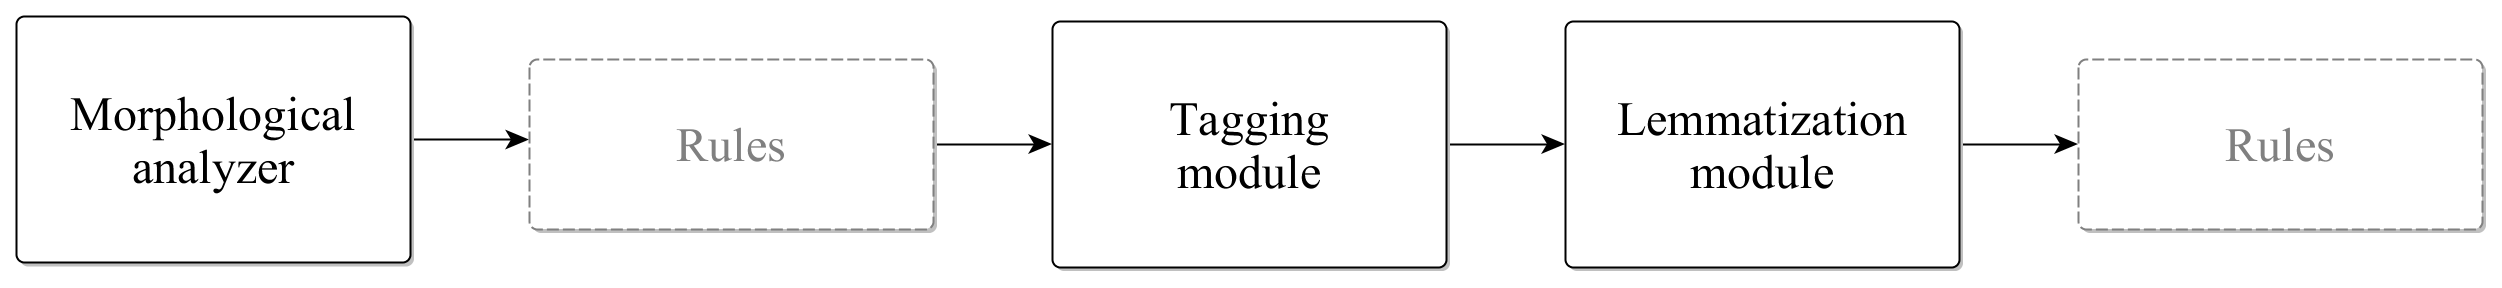
\includegraphics[width=1\textwidth]{MorphTagging/architecture.png} 
  \caption{The architecture of the full morphological tagging tool}
  \label{fig:purepos-arch_en}
\end{figure}

The architecture of PurePos (cf. Figure \ref{fig:purepos-arch_en}) is built up to allow multiple models cooperating effectively. 
In doing so, the disambiguation is carried out in multiple steps.
The data flow starts from a \acrshort{ma} providing word analyses as \emph{(lemma, tag)} pairs. 
Next, trigram-tagging methods (see \cite{Brants2000,Halacsy2007}) are employed for selecting morphosyntactic labels of words. 
In fact, these algorithms have been adapted to fit agglutinative languages.
Finally, lemmatization is carried out employing the methods presented in Thesis \ref{thes:morf-lemma}. 

\begin{figure}[H]
  \centering
  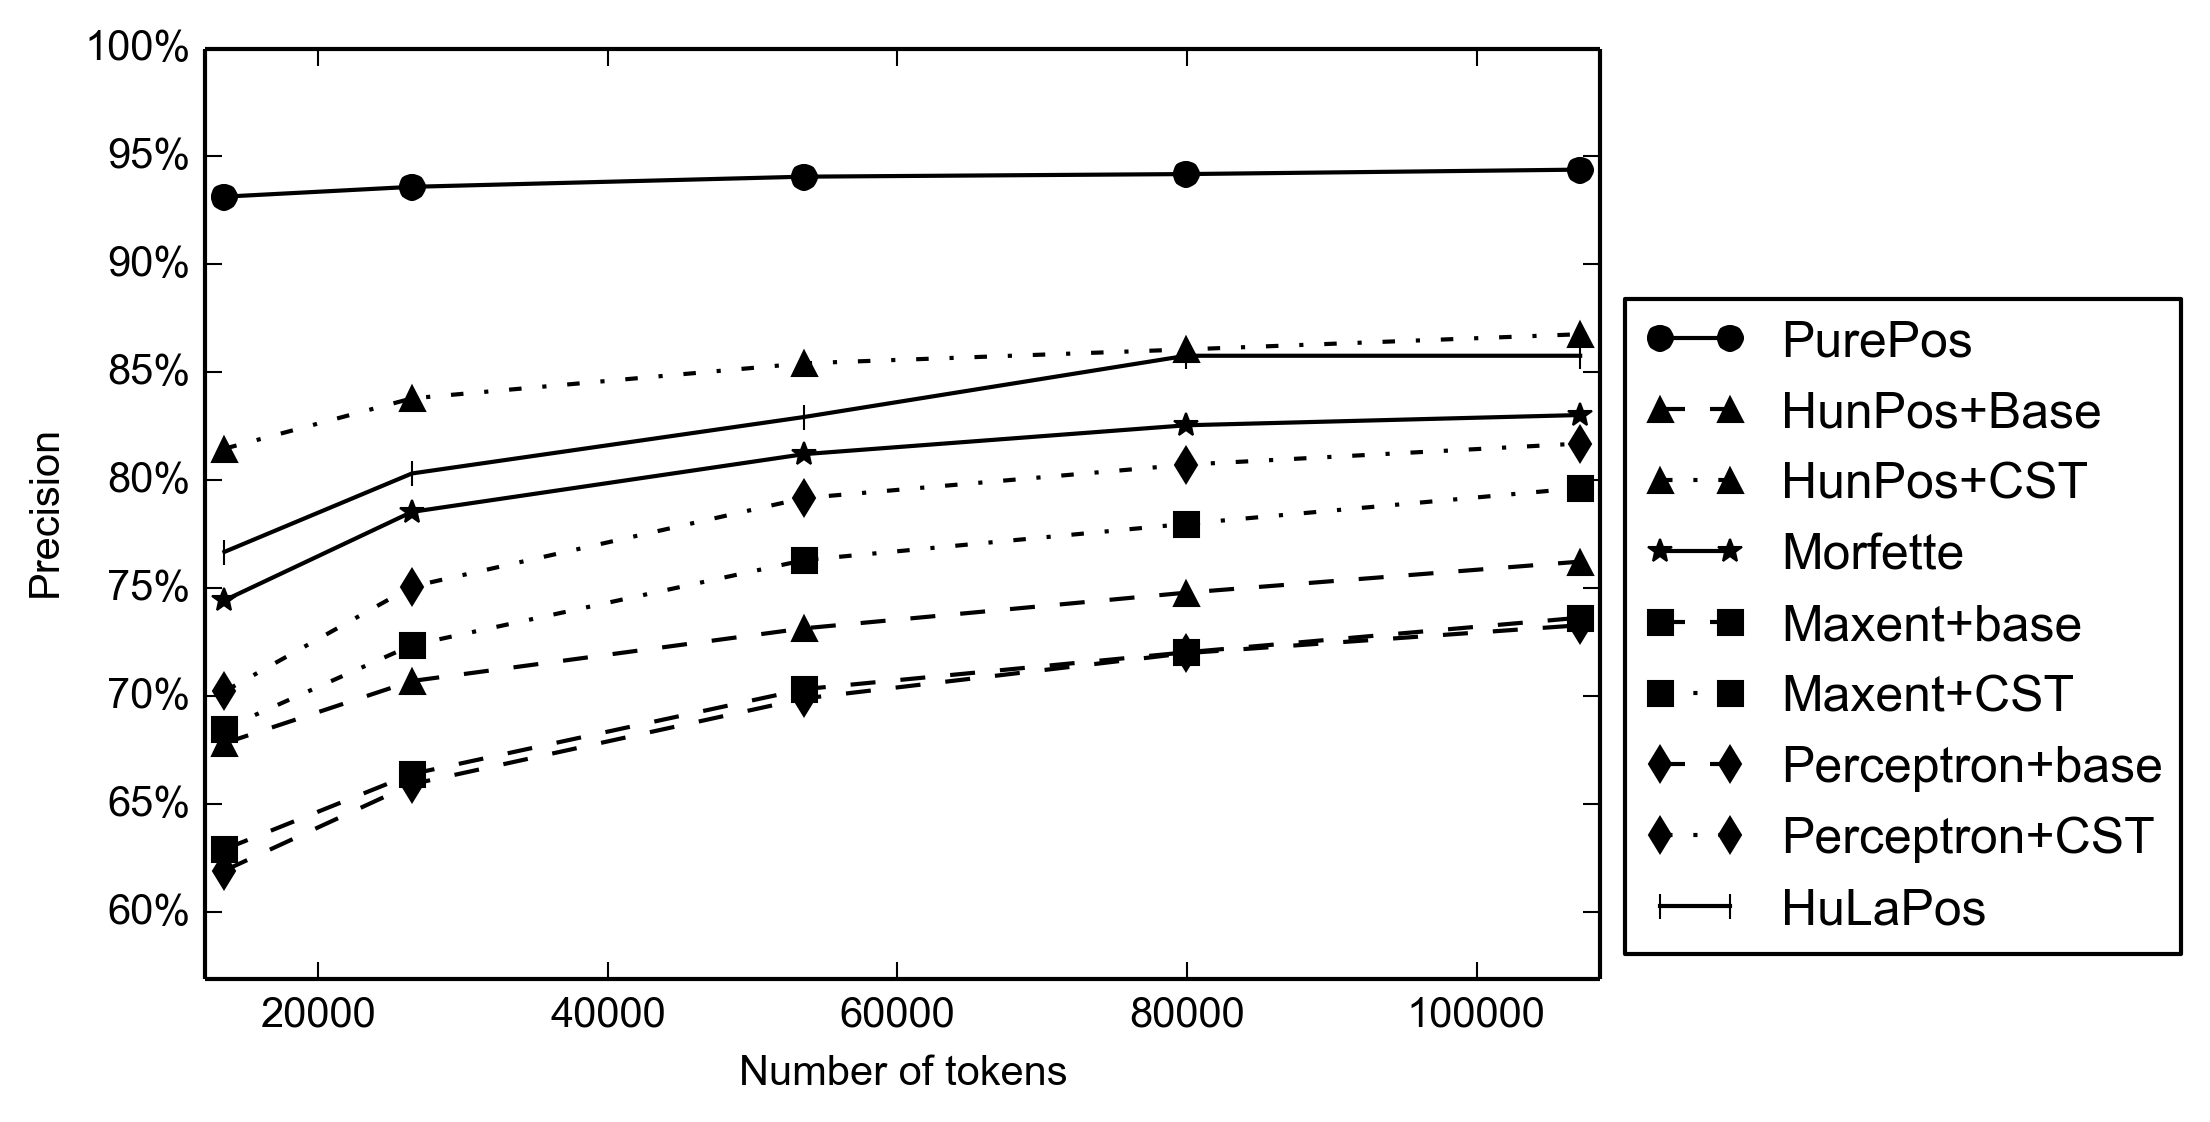
\includegraphics[width=1\textwidth]{MorphTagging/msd_token.png}
  \caption{Learning curves of full morphological taggers on the Szeged Corpus (using Humor labels)}
  \label{fig:humor-token_en}
\end{figure}

Several experiments are carried out measuring the performance of PurePos on the Szeged Corpus \cite{Csendes2004}.
Our results show that the new method yields 96.26\% full tagging accuracy, which it has the highest performance amongst available tools.
Moving on, we also compared existing tagging tools with ours on a less-resourced scenario.
These experiments show (cf. Figure \ref{fig:humor-token_en}) that PurePos can be successfully used even when the training data is limited.
Finally, all the hybrid enhancement of PurePos is evaluated one-by-one, showing that they can fix several sorts of errors.


\thesisline%%%%%%%%%%%%%%%%%%%%%%%%%%%%%%%%%%%%%%%%%%%%%%%%%%%%%%%%%%%%%%%%%%%%%

Although, methods presented in Thesis group \ref{thes:morf-tagging} have high accuracy, we show that they can be further improved.  
In the next, results are presented increasing the ceiling of morphological tagging tools' performance for agglutinative languages.


\begin{core}
\begin{thesis}
We developed a methodology for combining morphological tagging systems effectively.
The system presented selects the best lemma and tag candidates separately using two different combination schemes.
These components are trained with cross-validation using instance based methods.
We showed that our method can significantly reduce the errors of existing annotation tools.
\end{thesis}

\begin{pub}
\cite{Laki2013a,Orosz2013c,Orosz2013d} 
\end{pub}
\end{core}

First of all, discrepancy of tagging tools are investigated. 
For this, we designed a new metric (Own Error Rate) which measures the differences of taggers' output correctly.
In that way, we showed that the most typical mistakes of HuLaPos and PurePos are different enough to be aggregated.

Following this, the most common combination techniques are investigated considering their applicability to full morphological tagging.
A new combination method is presented involving adapted features sets for morphologically rich languages.
The novelty of our method is its architecture (cf. Figure \ref{fig:comb3_en}) which is able to compute full morphological annotations effectively.
The presented algorithm utilizes instance based learning \cite{Aha1991} and trains classifiers with cross-validation.
In doing so, it can utilize the whole training for both the baseline tools and the level-one learner.

\begin{figure}[H]
  \centering
  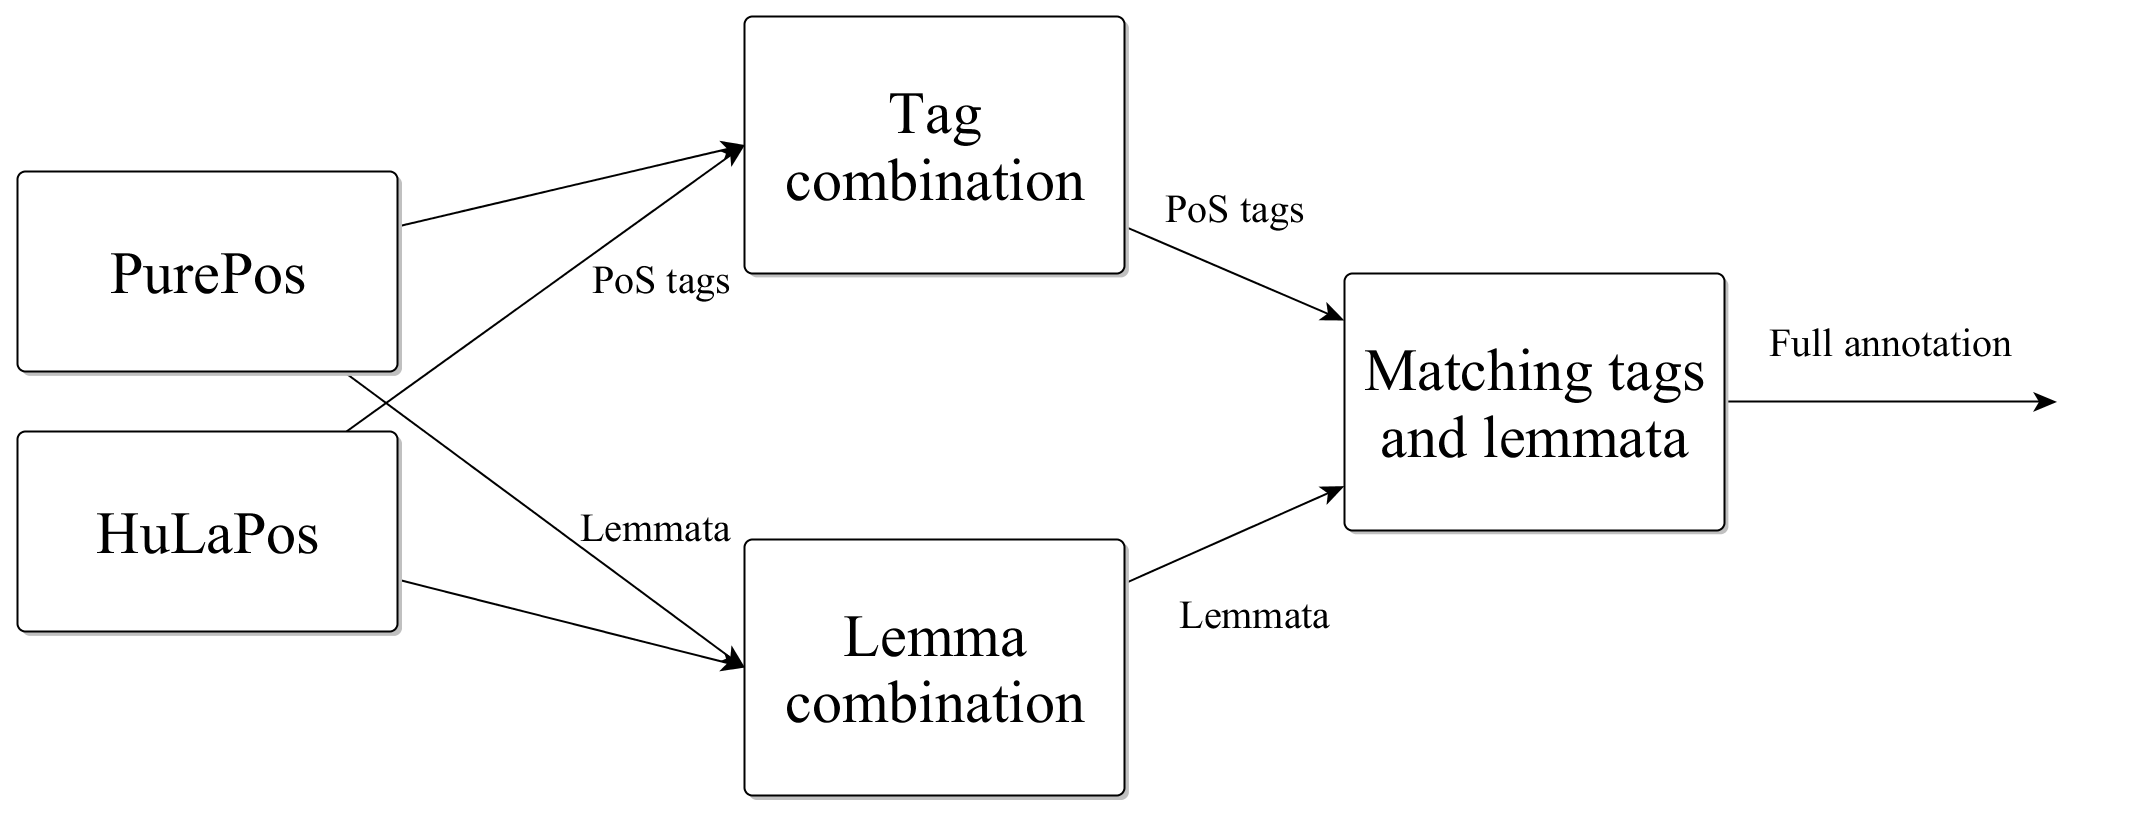
\includegraphics[scale=0.17]{MorphTagging/comb3.png} 
  \caption{Combining the output of two PoS taggers and lemmatizers}
  \label{fig:comb3_en}
\end{figure}


Finally, evaluation experiments are presented indicating that errors made by the best tagger can be further decreased.
The new algorithm resulted in 28.90\% error reduction rate compared to PurePos.

\subsection{Measuring morphosyntactic complexity using morphological annotation algorithms}
\label{thes:mlu}

Measuring morphosyntactic complexity plays and important role in linguistic studies, which is usually calculated in \acrlong{mlu}.
However, lengths of utterances are computed in morphemes (\acrshort{mlum}) for morphologically complex languages.
Although automatic methods and tools exist for e.g English, other less-resources languages lack of such systems.
Therefore, \acrshort{mlum} could be only computed manually, which is a time-consuming task.

This thesis group presents\footnote{This study is a joint work with Kinga Mátyus. 
%Manual annotation of the data were performed by both of us, while the morpheme counting principles are her work. 
My contribution is the construction of the tagging chain, its adaptation and the automatization of the MLUm calculation.} methods for processing speech transcripts effectively and estimating \acrlong{mlum} automatically.
%Our solution relies on the PurePos tagger tool (cf. Thesis \ref{thes:morf-tagging}).
%Results also indicate that the labor-intense manual work can be replaced with our new method.

\begin{core}
\begin{thesis}
\label{thes:spoken-morf-tagging}
We developed a hybrid morphological tagging chain for Hungarian speech transcripts.
Our method builds on top of the results presented in Thesis \ref{thes:morf-tagging}, adapting them to the domain.
Its evaluation shows that resulted performance is comparable with that of tagging methods for written corpora.
Moreover, our experiments indicate that the algorithm presented is accurate enough to be used in further applications.
\end{thesis}

\begin{pub}
\cite{Matyus2014,Orosz2014c}
\end{pub}
\end{core}

The proposed method adapts the algorithms introduced in Thesis \ref{thes:morf-tagging} for spoken Hungarian.
For this, analyses of the Humor \acrlong{ma} is augmented first with phenomena typical to the domain.
Next, the output of PurePos is adjusted utilizing domain-specific knowledge.

For this, a golden dataset of about 1,000 utterances from the \acrshort{hukilc} corpus is created containing manually verified morphological annotation. 
In doing so, a new tagging scheme is designed representing properly the characteristics of spoken language.
These manually corrected texts enabled us to develop and validate the proposed methods.

Evaluation of the chain resulted in 96\% token-level precision that is comparable with that of written taggers.
In that way, our investigation showed the PurePos is an appropriate base for tagging scenarios of spoken texts.

\thesisline%%%%%%%%%%%%%%%%%%%%%%%%%%%%%%%%%%%%%%%%%%%%%%%%%%%%%%%%%%%%%%%%%%%%%


\begin{core}
\begin{thesis}
\label{thes:mlu-estimation}
We proposed a new algorithm for estimating morphosyntactic complexity (calculating \acrlong{mlum}) in Hungarian speech transcripts.
The proposed method uses the morphological tagging chain of Thesis \ref{thes:spoken-morf-tagging} as a base.
In doing so, it computes lengths of utterances in its output.
Evaluation of the system indicates that our methodology can properly replace the time-consuming manual computation of human annotators.
\end{thesis}

\begin{pub}
\cite{Matyus2014,Orosz2014c}
\end{pub}
\end{core}

The estimation method analyzes morphological annotation of tokens.
Words known by the analyzer is decomposed by Humor, while length unknown words are guessed based on their \acrshort{pos} label.
This is followed by morpheme counting rules implementing linguistic guidelines, thus providing relevant estimates.

As regards resources, a manually checked corpus has been created for the experiments.
Evaluation results indicates that our approach highly correlates (0.9901) with counts of human annotators.
Further on, we have shown that the mean relative error of the method is only 4.49\%.
In that way, we have shown the proposed method can properly replace the labor-intense human computation.

\subsection{Effective preprocessing methods for a less-resourced noisy domain}
\label{thes:clin}

More and more electronic health records are produced in hospitals containing valuable but hidden knowledge.
Since doctors cannot spend enough time on writing them properly, notes often contain numerous errors.
Because of such mistakes, processing of them cannot be carried out using general-purpose tools.
Moreover, while several algorithms are becoming available for English, Hungarian and other morphologically rich languages are still neglected.

\begin{core}
\begin{thesis}%{II.1/b}
\label{thes:clin-segment}
We developed a new framework which segments noisy clinical records into words and sentences properly.
The method is built on top of well-known tokenization rules (e.g. \cite{Halacsy2004}), however, it augments them with unsupervised algorithms.
Evaluation experiments showed that the proposed tool can properly identify word and sentence boundaries in noisy clinical notes. 
Moreover, our results indicate that beside our approach none of the available systems can handle such error-full texts.
\end{thesis}

\begin{pub}
\cite{Orosz2013d, Orosz2014a}
\end{pub}
\end{core}

\begin{figure}[H]
  \centering
  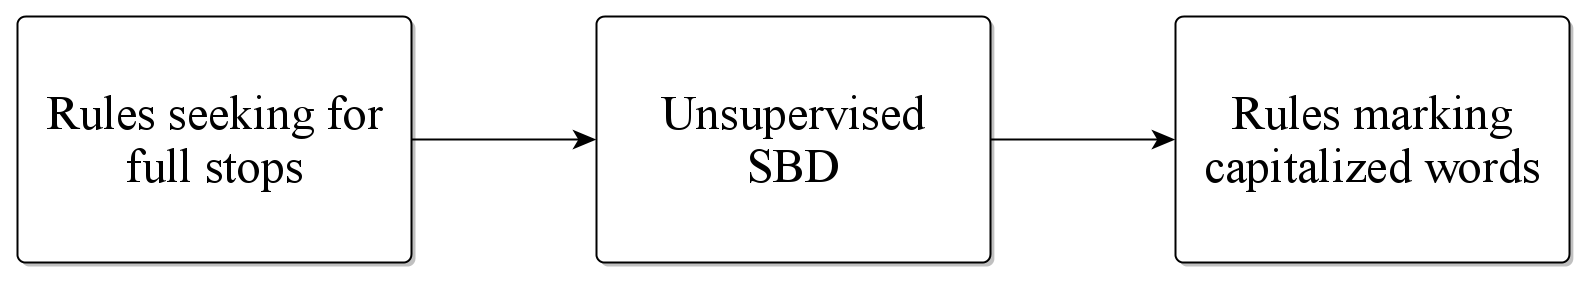
\includegraphics[scale=0.2]{Clinical/clin_segm_arch.png} 
  \caption{The architecture of the proposed method}
  \label{fig:clin-segment-arch_en}
\end{figure}

The proposed method builds on pattern-matching algorithms taken from general-purpose tokenization tools.
Even though these methods perform with high accuracy, their recall still stays low.
This study proposes a method (see Figure \ref{fig:clin-segment-arch_en}) which combines them with further unsupervised techniques.
In doing so, the scaled $\log\lambda$ filtering method \cite{kiss2006unsupervised} is adapted for the task by introducing new  factors.
Further on, the knowledge of a domain-specific morphological analyzer is utilized to fit the domain properly.

Evaluation of the framework is carried out on a manually segmented corpus. 
Numerous metrics (such as precision, recall, F-score) are employed measuring the performance of the proposed tool.
In doing so, we can analyze both the tokenization and the sentence boundary detection accuracy of the tool.
Besides, existing Hungarian systems are also compared with the proposed one.

Results show that existing systems can only produce low quality segmentation.
Moreover, most of them result in F-scores less than 50\% concerning sentence boundary identification.
On the contrary, the presented method can detect both token and sentence boundaries properly, producing F-values over 90\%.


%%%%%%%%%%%%%%%%%%%%%%%
\thesisline%%%%%%%%%%%%
%%%%%%%%%%%%%%%%%%%%%%%

\begin{core}
\begin{thesis}%{II.2}
\label{thes:clin-pos}
We showed that tagging methods of Thesis \ref{thes:morf-tagging} can be modified for annotating electronic health records properly.
In doing so, PurePos is adjusted with stochastic and symbolic domain adaptation techniques.
Evaluation results indicate that the quality of the annotation produced is comparable with that of general written tagger tools.
\end{thesis}

\begin{pub}
\cite{Orosz2013,Orosz2014b} 
\end{pub}
\end{core}

We use an extended version of the Humor analyzer as a base. 
This tool has been prepared\footnote{The lexicon extension is carried out by Attila Novák \cite{Orosz2014} .} to analyze electronic health records properly.
Further on, the tagging chain is improved using a detailed error analysis of the baseline tagging chain.

For this, a manually annotated corpus is created containing texts of clinical notes.
Results show that the improved system performs significantly better (93.73\%) than the baseline system used (88.09\%).
However, future work might target the segmentation and tagging problem with a unified framework, since both systems have the most issues with abbreviated terms.

\let\thesubsection=\oldthesubsection